\documentclass{article}

\usepackage[a4paper]{geometry} % document dimensions
%\usepackage{amsmath} % multiline equation numbering
\usepackage{amssymb} % e.g. triangleq, checkmark
\usepackage{textcomp,gensymb} % \degree symbol
%\usepackage{bm} % bold symbols numbering
\usepackage{authblk} % author/affiliation block
\usepackage[T1]{fontenc} % support accents via UTF
\usepackage[titletoc,title]{appendix}

\usepackage{graphicx} % support for graphics
\usepackage[hidelinks, backref=page]{hyperref} % hyperlinks and autoref
\hypersetup{
    pdfauthor={Nick Ackerley},
    pdfsubject={Engineering Seismology},
    pdftitle={Open Model of Probabilistic Seismic Hazard Assessment for the Indian Subcontinent},
    pdfkeywords={seismology, hazard, India, OpenQuake}}
\usepackage{natbib} % bibliography support
\usepackage{adjustbox} % support for too-wide figures
\usepackage{caption} % support for captions of floats
\usepackage{capt-of} % support for captionof
\usepackage{subcaption} % support for multiple figures with captions
\providecommand*\hyphen{-} % dashed page numbers in bib
\usepackage{listingsutf8} % for syntax-highlighted code
\usepackage[usenames,dvipsnames]{xcolor} % e.g. RoyalBlue
\usepackage{fontspec} % support for setmonofont
\setmonofont{Ubuntu Mono}[Scale=MatchUppercase]

%\usepackage{multirow} % cells spanning rows in tables
%\usepackage{array} % vertically aligned table cells

\usepackage{enumitem} % control list formatting
\setlist[2]{nosep}

% allow figures to take up more of a page
\renewcommand{\floatpagefraction}{0.7}

% set up back-references
\renewcommand*{\backref}[1]{}
\renewcommand*{\backrefalt}[4]{%
    \ifcase #1 (Not cited.)%
    \or        (Cited on page~#2.)%
    \else      (Cited on pages~#2.)%
    \fi}

\lstdefinelanguage{Ini}
{
    basicstyle=\ttfamily\footnotesize,
    breaklines=true,
    keepspaces=true,
    columns=fullflexible,
    morecomment=[s][\color{RoyalBlue}\bfseries]{[}{]},
    morecomment=[l]{\#},
    morecomment=[l]{;},
    commentstyle=\color{gray}\ttfamily,
    morekeywords={},
    otherkeywords={=,:},
    keywordstyle={\color{green}\bfseries},
}

%%% PREAMBLE

\begin{document}

\title{Open Model of Probabilistic Seismic Hazard Assessment for the Indian Subcontinent}
\date{\today}

\setcounter{Maxaffil}{0} % compact author block
\author[1,2]{N. Ackerley}
%\author[3]{G. Weatherill}
%\author[3]{M. Pagani}
\affil[1]{Istituto Universitario di Studi Superiori, Pavia, Italy}
\affil[2]{Université Joseph Fourier, Grenoble, France}
%\affil[3]{Global Earthquake Model (GEM), Pavia, Italy}

\maketitle

\begin{abstract}
Open models encourage peer review and collaboration; open models can be built upon.
\end{abstract}

\tableofcontents
\listoffigures
\listoftables

\section{Introduction}
\label{sec:Introduction}

In this work a seismic hazard model for peninsual India \cite{nath2012probabilistic} has been implemented under the OpenQuake \citep{weatherill2014openquake,crowley2015openquake} platform.

File names in the published model are shown in \texttt{typewriter} font, as are keywords specific to OpenQuake, such as \texttt{bGRRelative}.

\subsection{Seismic hazard in peninsular India}
\label{sec:PshaIndia}

\subsection{Open science and OpenQuake}
\label{sec:Open}

\section{Model implemetation}
\label{sec:Model}

\subsection{Seismogenic sources}
\label{sec:Sources}

\cite{thingbaijam2011seismogenic}

\subsubsection{Areal sources}
\label{sec:Areal}

As we will see in \autoref{subsubsec:GmpeTree} ground motion prediction logic trees depend on correct assignment of tectonic region types. The main difficulty in implementing the areal source model of  \cite{nath2012probabilistic} was that although their intentions were generally clear, these assignments were not made explicit. Tectonic region type assignments were therefore made using a combination of the representative focal mechanisms reported by \cite{nath2012probabilistic} and fault maps such as the HimaTibetMap database \citep{styron2010database}. Since the representative focal mechanism was computed as the average of the moment tensors reported in the GCMT database weighted by magnitude it is biased in favour of the larger earthquakes \citep{thingbaijam2011seismogenic}. The inferred tectonic region assignments assumed are shown in \autoref{fig:ArealSourceModel}.

\begin{figure}[!htb]
\begin{adjustbox}{center}
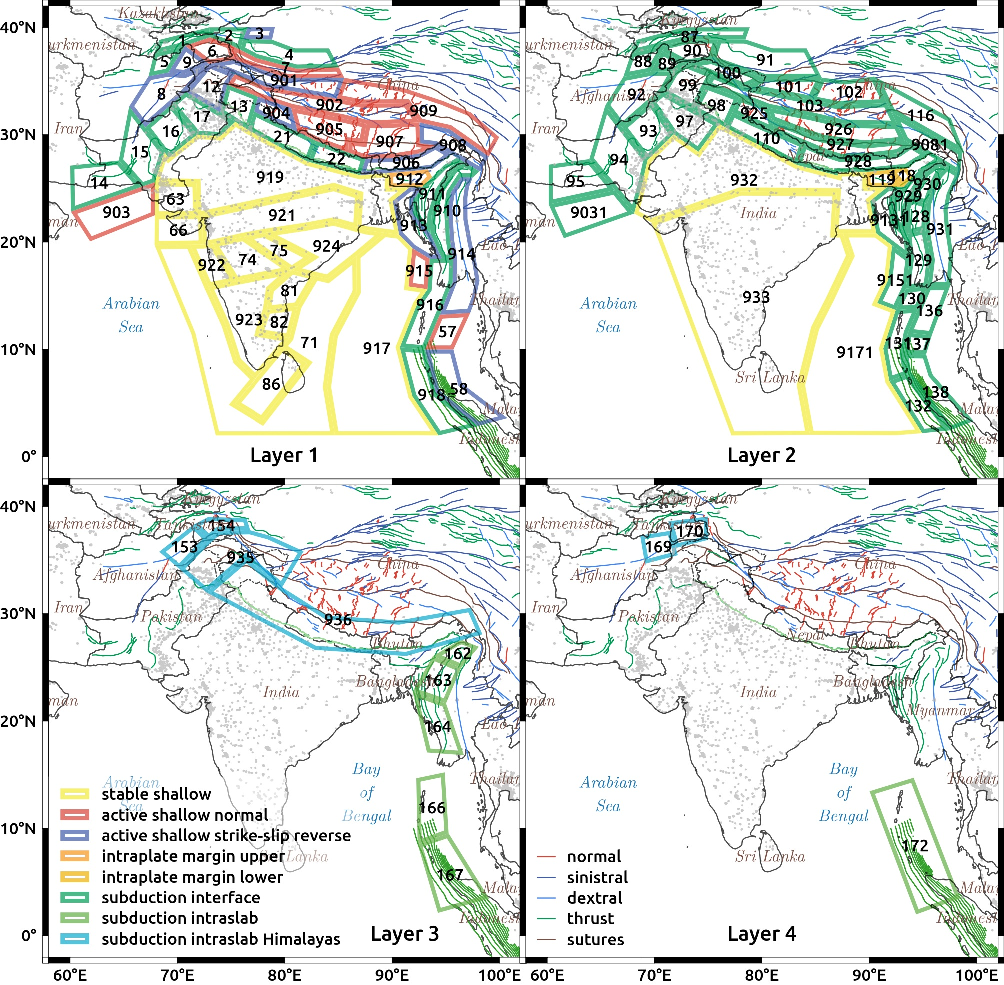
\includegraphics{India_Areal_Source_Model}
\end{adjustbox}
\caption[Areal source model]{Areal source model tectonic region assignments used in GMPE logic tree. The areal source models is encoded in \texttt{areal\_source\_model.xml}. Zone identification numbers from \cite{nath2012probabilistic} are indicated. Fault traces are from HimaTibetMap-1.0 \citep{styron2010database} except the Sumatran subduction fault which is from SLAB~1.0 \citep{hayes2012slab1}. Fault data from the stable regions of India is lacking. Urban areas, ``contiguous patches of built-up land greater than 1~km²'' \citep{schneider2009new}, are indicated in darker grey.}
\label{fig:ArealSourceModel}
\end{figure}

Potentially problematic tectonic region type assignments:
\begin{itemize}
\item zone 906 in the Great Himalayas just north of the Shillong plateau was assigned ``active shallow crust strike-slip reverse'' even though the main trace of the Himalayan subduction fault runs through it, because the representative focal mechanism is strike-slip. 
\item zones 71, 86 on layer 1 and zones 9031, 9081, 9131, 9151 and 9171 on layer 2 have have $a$ values of zero and so were not included in the areal source model
\end{itemize}

Magnitude-scaling relations were selected based on the same source zonation, since ``Wells and Coppersmith (1994) for crustal events and those given by
Strasser et al. (2010) for the subduction earthquakes'' \citep[p.~140]{nath2012probabilistic}. For interface and intraslab regions \texttt{StrasserInterface} and \texttt{StrasserIntraslab} were used, respectively. 

The comment that ``the fault-rupture area estimated from the magnitude is constrained by a factor of 2'' \citep[p.~140]{nath2012probabilistic} is interpreted as a width/depth aspect ratio of 2.

The seismogenic depth was assumed to be midway between the minimum and maximum. Is this justified by \cite{thingbaijam2011seismogenic}? Could it stand further refinement?


\subsubsection{Smoothed seismicity}
\label{sec:Smoothed}

Each point in the smoothed seismicity model was treated as a point source. \cite{nath2012probabilistic} have provided ``spatially varying annual activity rates while b-value and m max remain fixed within the source zone''. Thus for the smoothed seismicity model the parameters $b$ and $M_{max}$ of the truncated Gutenberg-Richter magnitude-frequency distributions are to be inferred from the areal source model zonation. For points inside zones with non-zero $a$ values in the areal source model this is trivial; for points outside these zones the zone with the shortest perpendicular distance was chosen.

A point source model in OpenQuake also requires definition of the uncertainty of the probability distribution, as well as the tectonic region type and source mechanism for the selection and implementation of GMPEs, respectively. Thus the same procedure was used to assign $\sigma_b$, $\sigma_{m_{max}}$, tectonic subregion, rake, dip, strike and magnitude scaling relations were used.

The electronic supplement to \cite{nath2012probabilistic} for the smoothed-gridded seismicity models simply gives values for \texttt{nu4\_5} and \texttt{nu5\_5} for each latitude and longitude, where ``$\nu_i$ , is the annual activity rate for $i$th seismogenic source for a threshold magnitude'' \cite[p.~140]{nath2012probabilistic}.

The truncated Gutenberg-Richter magnitude-frequency distribution in OpenQuake implements
$$\lambda(M \geq m) = 10^{a - b m} = e^{\alpha - \beta m}$$
where, since $\lambda$ is an annual rate, $10^a$ is too. If we ignore events below some threshold $m_{min}$ then the annual rate becomes
$$\lambda(M \geq m_{min}) = e^{\alpha - \beta m_{min}} e^{-\beta (m - m_{min})} = \nu e^{-\beta (m - m_{min})} $$
Thus to compute the $a$ value required by OpenQuake from the activity rate $\nu$ for a given magnitude threshold, we must also take into account the $b$ value for the zone:
$$a = \log_{10}(\nu) + b m_{min}$$
[It would be good to cite a reference here. Is a correction for bin size necessary?]

\begin{figure}[!htb]
\begin{adjustbox}{center}
\includegraphics{India_Smoothed_Source_Model}
\end{adjustbox}
\caption[Smoothed seismicity point source model]{Tectonic region assignments and activity rates for smoothed seismicity point source model. The smoothed seismicity source models are encoded in \texttt{smoothed\_source\_model\_mmin4.5.xml} and \texttt{smoothed\_source\_model\_mmin5.5.xml}}
\label{fig:SmoothedSourceModel}
\end{figure}

Other assumptions:
\begin{itemize}
\item zones 9031, 9081, 9131, 9151 and 9171 on layer 2 have $m_{max}$ values values of zero so the the smoothed seismicity points in or nearest to these zones on layer 2 were assigned the $m_{max}$ values from the corresponding zones on layer 1, namely zones 903, 908, 913, 915 and 917.
\end{itemize}

Note differences in grids: although the hazard maps in the electronic supplement are at 0.2° and the paper says the smoothed-gridded models are also at 0.2° they are in fact at 0.1°. Figure shows the model at just 0.2°.

Note smoothing details. A Gaussian kernel is used, following the methodology of \cite{frankel1995mapping} with correlation distances of 65 and 85~km for $m_{min}$ of 4.5 and 5.5 respectively. The method involves smoothing event counts, thus events per year, for a given minimum magnitude.

\subsection{Ground-motion prediction}
\label{sec:GroundMotion}

\cite{sharma2009ground} points out that the decay rate of PGA for shallow India-Bangladesh and deep India-Burma border events have different distance scaling. The former leads to the necessity of a GMPE specific to the Shillong plateau \cite{nath2012ground} while the latter means interface subduction events need to be treated differently. 

Issues encountered while implementing GMPE logic tree:
\begin{itemize}
\item layer~4 depth range of 180-300~km is significantly deeper than deepest events used in regression for ATBO03 (100 km), LILE08 (161 km), ZHAO06 (120 km) and GUPT10 (148 km) are specified for. YCSH97 only included events to 229 km. KANN06 is specified to 200 km depth, but is only used for interface events (layer~2).
\item Assumed “and Andaman-Sumatra subduction” missing from Figure 3.
\item Why is Youngs (1997) not used in the subduction interfaces?
\item Should the Japan/Cascadia distinction not also be used for interface subduction with Atkinson \& Boore (2003)?
\item \cite{nath2012probabilistic} doesn't seem to me to follow the recommendations of \cite{nath2011peak} as far as having two subduction intra-slab sub-regions: the former uses Indo-Myanmar and Himalayas while the latter recommends Indo-Myanmar and Hindukush. \cite{nath2012probabilistic} is followed strictly for for phase 1.
\item Assignment of source mechanism (normal or not, matters in shallowest layer only) is tricky.  Dip cannot be used to distinguish normal and reverse subduction because the subduction interface angle is not known. different GMPEs use different rake thresholds; a threshold of 30\degree\space was chosen, consistent with \cite{boore2008ground, campbell2008nga} but not \cite{zhao2006attenuation}.
\end{itemize}

Issued encountered while implementing GMPEs:

\cite{sharma2009ground}
\begin{itemize}
\item lacks a $M^2$ term \cite{cotton2006criteria}
\item does not define rock vs. soil
\end{itemize}

\cite{raghukanth2007estimation}
\begin{itemize}
\item typographical errors in coefficient tables: grossest error fixed, 3 other errors causing approximately 10\% error not fixed
\item actually defines 4 different models: must assume that for all of peninsular India was used by \cite{nath2012probabilistic}, not one of those for sub-regions.
\end{itemize}


\begin{table}
\caption[Ground motion prediction equations]{Ground motion prediction equations. Models newly implemented in OpenQuake as part of the current work are indicated.}
\label{table:GMPE}
\centering
\begin{tabular}{c c l}
\hline
 Code & New & Reference \\
\hline
 AKBO10 & & \cite{akkar2010empirical} \\
 BOAT08 & & \cite{boore2008ground} \\ 
 CABO08 & & \cite{campbell2008nga} \\ 
 ZHAO06 & & \cite{zhao2006attenuation} \\ 
 ATBO03 & & \cite{atkinson2003empirical} \\ 
 ATMA09 & & \cite{atkinson2009predicted} \\ 
 LILE08 & & \cite{lin2008ground} \\ 
 YCSH97 & & \cite{youngs1997strong} \\ 
 TORO02 & & \cite{toro2002modification} \\ 
 ATBO06 & & \cite{atkinson2006earthquake} \\ 
 CAMP03 & & \cite{campbell2003prediction} \\ 
 SDBK09 & \checkmark & \cite{sharma2009ground} \\
 RAIY07 & \checkmark & \cite{raghukanth2007estimation} \\
 NTMN12 & \checkmark & \cite{nath2012ground} \\
 GUPT10 & \checkmark & \cite{gupta2010response} \\
 KNMF06 & \checkmark & \cite{kanno2006new} \\
\hline
\end{tabular}
\end{table}

\subsection{Logic Trees}
\label{subsec:LogicTrees}

\subsubsection{Ground-Motion Prediction}
\label{subsubsec:GmpeTree}

The GMPE logic tree implemented in \cite{nath2012probabilistic} is shown in \autoref{fig:GmpeTreeNath}. Since some of these GMPEs are new to OpenQuake (see \autoref{table:GMPE}) a comparison was done between that model and that obtained with only the standard GMPEs. For this purpose a "simplified" GMPE logic tree was constructed which simply omitted the newly-implemented GMPEs and retained equal weighting for the rest.

\begin{figure}[!htb]
\begin{adjustbox}{center}
\includegraphics{gmpe_logic_tree.pdf}
\end{adjustbox}
\caption[Simplified GMPE logic tree]{Simplified GMPE logic tree employing only established OpenQuake models, as encoded in \texttt{gmpe\_logic\_tree.xml}. Middle column selects tectonic region types as defined in \autoref{fig:ArealSourceModel}. OpenQuake model class names and assigned weights are given on the right side. New and established models are enumerated in \autoref{table:GMPE}}
\label{fig:GmpeTreeSimplified}
\end{figure}

\begin{figure}
\begin{adjustbox}{center}
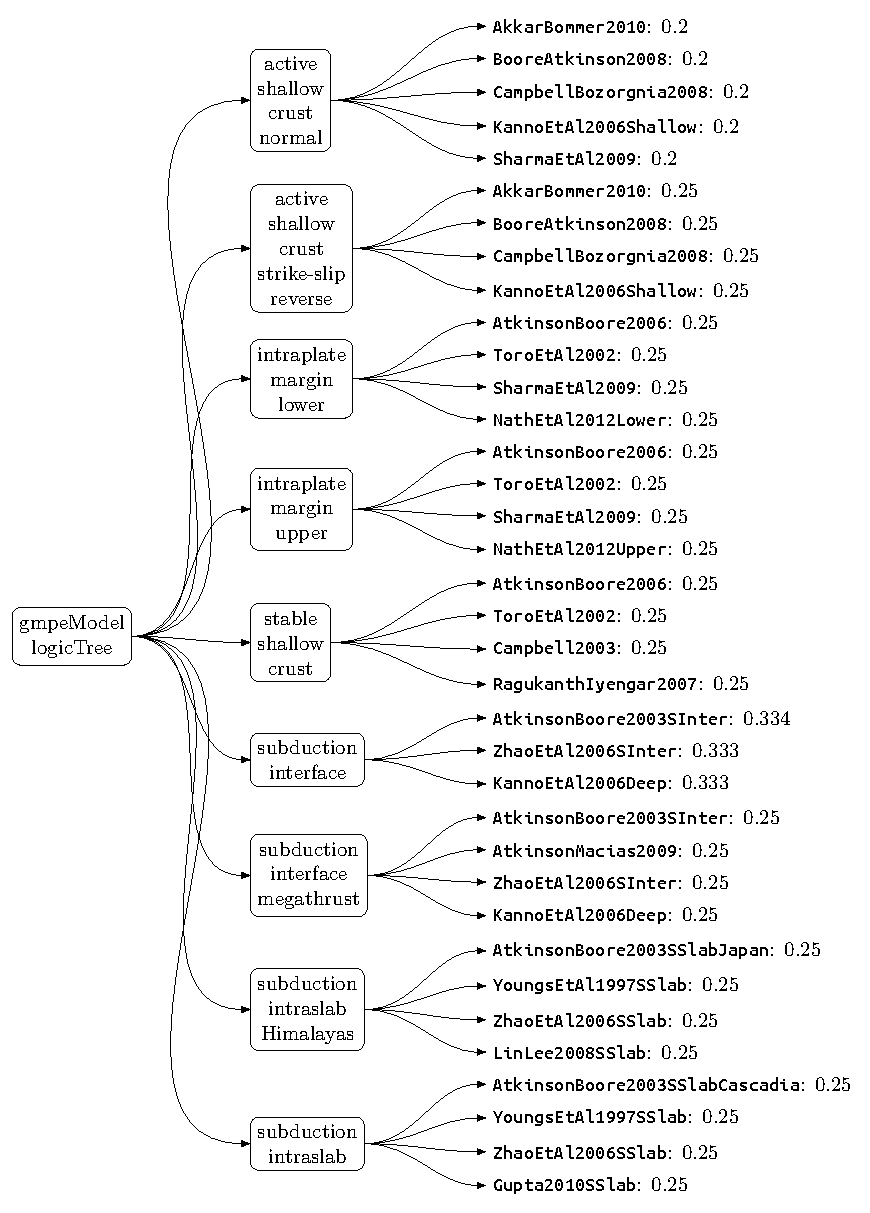
\includegraphics{gmpe_logic_tree_all.pdf}
\end{adjustbox}
\caption[Original GMPE logic tree]{GMPE logic tree of \cite{nath2012probabilistic}, as encoded in \texttt{gmpe\_logic\_tree\_all.xml}. See \autoref{fig:GmpeTreeSimplified} for more commentary}
\label{fig:GmpeTreeNath}
\end{figure}

Moving forward an obvious modification is to replace superseded NGA models with their more up-to-date versions. 

[It may also be desirable to rationalize the weighting of the GMPEs or include entirely new ones, such as the new BC Hydro subduction model \citep{abrahamson2012bc}. The discussion continues below and is incomplete.]

\cite{anbazhagan2015selection} seem to be proposing different weights for different regions based on single events in those regions. An extreme example is to define different weights for Anjar, 1956 and Bhuj , 2001 earthquakes even though the epicentres and depths were very close together. In contrast \cite{nath2011peak} compute LLH for 7 regions (using 38 events total) and state that, ``individual events do not have significant number of observations to support a viable ranking basis.''

\cite{anbazhagan2015selection} seem to misuse the concept of data support index (DSI) \citep{delavaud2012toward} by setting weights to zero when the DSI is negative. The threshold is arbitrary and is chosen without discussion. As \cite{delavaud2012toward} point out ``more important
than the sign of the DSI is the difference of DSI between
two models.''

Both \cite{anbazhagan2015selection} and \cite{nath2011peak} rely on estimating ground motions from macroseismic intensity. I'm sure it is a matter of low seismicity and lack of instrumentation, but I'm still surprised. I would expect the catalogue for peninsular India to be complete for 20 years to magnitude 5 so that one could thus get 10 well-recorded events, at least. There is significant additional (aleatory and epistemic) variability in mapping EMS to PGA which must obscure the true performance of the GMPEs.  Perhaps this is part of why  \cite{anbazhagan2015selection} and \cite{nath2011peak} arrive at such different LLH scores and rankings for the same events \cite[][Table 5]{anbazhagan2015selection}. It would be interesting to compare the results of LLHs computed using EMS inferred from digitized intensity maps to those computed using instrumental PGA for at least a few events since 1990. \cite{nath2011peak} take a step towards this by looking at the scatter in their mapping of PGA to EMS but it's not quite the same.

Many authors \citep{scherbaum2009model, nath2011peak, delavaud2012toward, anbazhagan2015selection} seem unduly interested in "ranking", i.e.  constructing an ordered list of GMPEs. This is not a horse race. \cite{scherbaum2009model} suggests a way to turn an LLH score into a logic-tree weight and the formula does not require ranking. Furthermore, in constructing a logic tree one must include factors outside the performance-based scoring, for example an assessment of whether the set is ``mutually exclusive and collectively exhaustive'' \citep{bommer2008use}. For me the question of ranking is just "noise" which obscures more important questions.

The mutual exclusivity requirement means, to me, that models should be omitted which are redundant in the sense of being too similar to other models in terms of the methodology of their construction, especially if that means they make similar predictions and have similar limitations as a result. For example the exclusion of models which have been superseded \citep{cotton2006criteria} can be seen as an application of the requirement that models be mutually exclusive. Another example would be, for a GMPE logic tree intended for the Indian subcontinent, to omit a model such as \cite{hwang1997attenuation} in favour of \cite{atkinson2006earthquake} since both are based on stochastic simulation in Eastern North America.

The collective exhaustiveness requirement means, is trickier. It is this requirement which pushes hazard modellers to seek out and evaluate more and complementary types of models. Thus models with broad data support from other regions complement models with poor data support from the target region. Stochastic models supplement data-driven models. Models with different functional forms, distance or magnitude ranges can complement each other.

The process of developing a logic tree to assess epistemic uncertainty is thus a dialectical one. Mutual exclusivity and collective exhaustiveness comprise opposing forces which must be exerted alternately and in tandem.

[Now apply these principles to move forward from \cite{nath2012probabilistic}!] 

\subsubsection{Source Models}
\label{subsubsec:SourceTree}

The source model logic tree is shown in symbolic form in \autoref{fig:SourceTreeSymbolic}.

\begin{figure}[!htb]
\begin{adjustbox}{center}
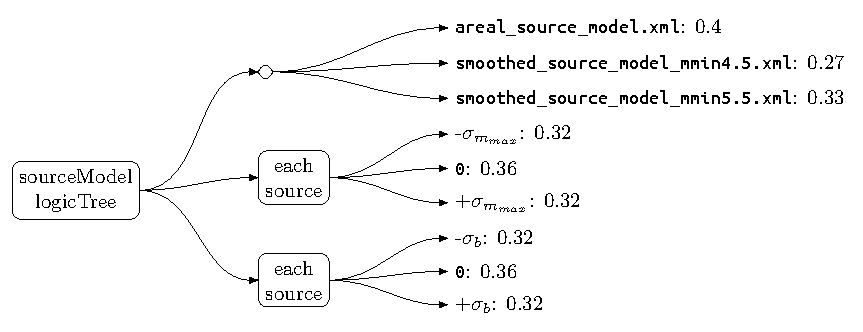
\includegraphics{source_model_logic_tree_simplified.pdf}
\end{adjustbox}
\caption[Symbolic source model logic tree]{Symbolic source model logic tree of \cite{nath2012probabilistic}.}
\label{fig:SourceTreeSymbolic}
\end{figure}

\cite{nath2012probabilistic} accounts for the epistemic uncertainty in seismicity model parameters by estimating the standard deviations of $b$ and $m_{max}$ in each source zone and assigning weights to ±1 standard deviation for each source. This results in a source model logic tree too large to represent on a page; just a portion of it is shown in \autoref{fig:SourceTreePartial}. 

\begin{figure}
\begin{adjustbox}{center}
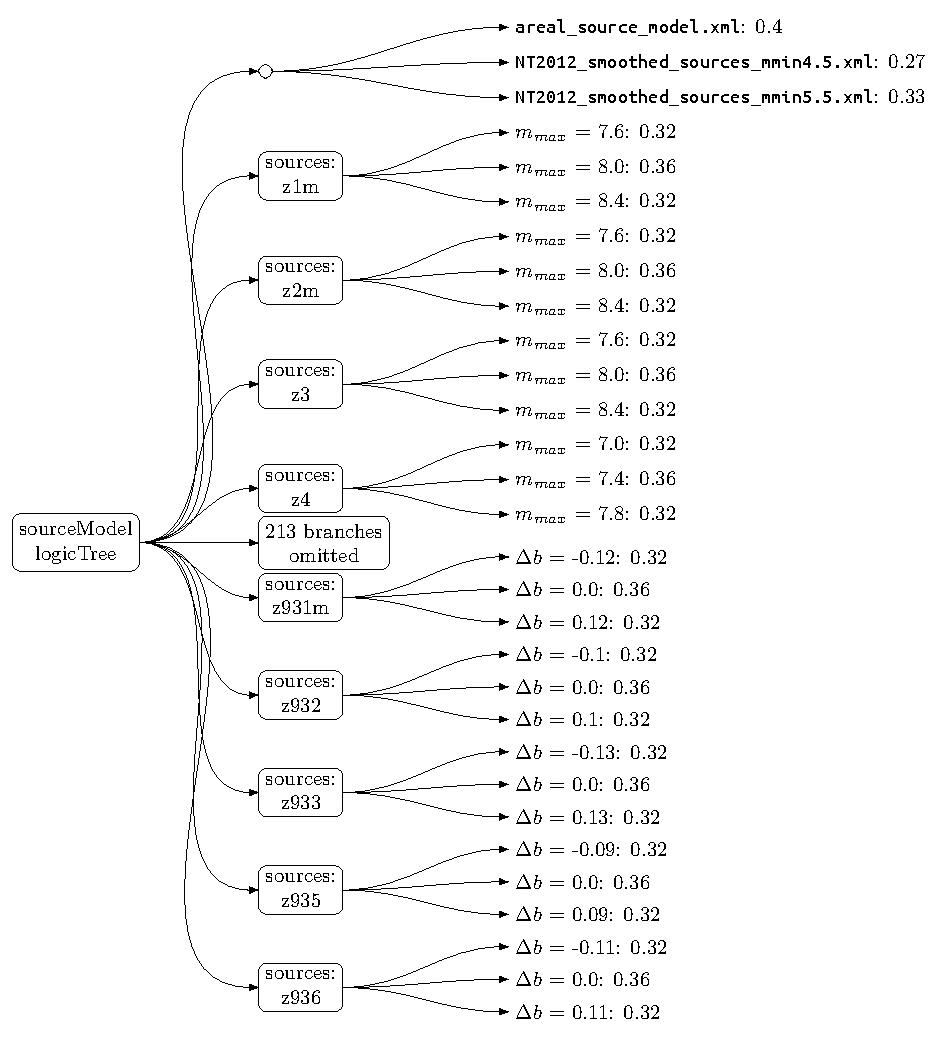
\includegraphics{source_model_logic_tree.pdf}
\end{adjustbox}
\caption[Partial source model logic tree]{Partial source model logic tree of \cite{nath2012probabilistic}. The full model is encoded in \texttt{source\_model\_logic\_tree.xml}}
\label{fig:SourceTreePartial}
\end{figure}

Note that although Figure 4 of \cite{nath2012probabilistic} shows the activity rate $\nu$ (and by implication $a$) varying with $b$, no estimates of the standard deviation of $a$ or $nu$. The  in OpenQuake happens to recalculate $a$ as $b$ After modifying $b$ using the uncertainty type \texttt{bGRRelative} the $a$ value is automatically recalculated to maintain constant total moment rate. It has been assumed that this is the behaviour which \cite{nath2012probabilistic} implemented.

\section{Hazard results}
\label{sec:Hazard}

\subsection{Verification}
\label{sec:Verification}

\subsection{Sensitivity}
\label{subsec:Sensitivity}

\section{Conclusions}
\label{sec:Conclusions}

\section*{Acknowledgement}
Acknowledgements here

\bibliographystyle{apalike}
\bibliography{/home/nick/Desktop/Library/PSHA.bib}

\begin{appendices}

\section{}
\subsection{Job Configuration Files}
\label{ch:Jobs}

\lstinputlisting[language=Ini,caption=\lstname]{phase1.ini}

\end{appendices}

\end{document}